\documentclass{crypto-exercise}
\usepackage{pgfplots}
\author{Sven Laur}
\contributor[Write down the initial solution]{Ivo Kubjas}
\editor{Sven Laur}
\tags{Discrete Logarithm problem, random self-reducibility, missing solution, time-success profile}
\begin{document}

\newcommand{\XS}{x_{*}}
\newcommand{\XZ}{x_{0}}
\newcommand{\XGUESS}{x_{\text{guess}}}
\newcommand{\YZ}{y_{0}}
\newcommand{\TMAX}{t_{\mathrm{max}}}


\begin{exercise}{Random self-reducibility of DL}
  Let $\GG=\langle g\rangle$ be a finite group of an order $q$
  generated by the powers of an element $g$. Then the Discrete
  Logarithm (DL) problem is following. For any element $y$ find a
  power $x\in\ZZ_q$ such that $g^x=y$. The advantage of an discrete
  logarithm finder $\AD$ is defined as
  $\ADVDL{\GG}{\ADB}=\pr{\BGAME^\ADB=1}$ where the corresponding
  security game is 
  \begin{align*}
    \begin{game}{\BGAME^\ADB}
      & x \getsu \ZZ_q\\
      & \RETURN [x \iseq \ADB(g^x)]\enspace.
    \end{game}
  \end{align*}
  \begin{enumerate}
  \item Show that Discrete Logarithm problem is random self-reducible,
    i.e., for any algorithm $\ADB$ there exists an oracle algorithm
    $\AD^{\ADB}$ that for any input $y\in\GG$ outputs the correct
    answer with the probability $\ADVDL{\GG}{\ADB}$ and has roughly
    the same running time.
  \item Given that the DL problem is random self-reducible, show that
    the difficulty of DL instances cannot wary a lot. Namely, let
    $\ADB$ be a $t$-time algorithm that achieves maximal advantage
    $\ADVDL{\GG}{\ADB}$. What can we say about worst-case advantage
    \begin{align*}
      \min_{y\in\GG}\pr{x\gets\AD(y): y=g^x}?
    \end{align*}
    Can there be a large number of inputs $y$ for which the DL problem
    is easy?
  \item Show how to amplify the success rate of $\ADB$ by
    repetitions. Sketch the corresponding time-success profile
    $\varepsilon(t)$. What does this say about time-success profile of
    DL problem in general?
  \end{enumerate}
\end{exercise}

\begin{solution}
\textsc{Random Self-reducibility.}
First, note that we can use `pick $x \getsu \ZZ_q$ and set $y\gets g^x$ and `pick $y \getsu \GG$' interchangeably. As $g$ is a generator of $\GG$, then for uniformly sampled $\XZ$ we get that $y = g^{\XZ}$ is also uniform in $\GG$ because $g$ generates all elements in $\GG$ exactly once. On the other hand, for uniformly sampled $\YZ$ there is exactly one $\XZ \in \ZZ_q$ such that $y = g^{\XZ}$. Now by the assumptions of the exercise the advantage for the adversary $\ADB$ is
  \begin{align}
  \ADVDL{\GG}{\ADB} = \pr{\BGAME^\ADB=1} = \pr{x\gets \ZZ_q: x=B(g^x)}
  \label{adv_b}.
\end{align}
However, the latter holds only if the challenge power $x$ is uniformly sampled from $\ZZ_q$. Hence, we need to construct an algorithm $\AD$ that feeds $\ADB$ with uniformly chosen group elements but on the same time can utilise the results. We construct the adversary $\AD^\ADB$ as follows:
  \begin{align*}
    \begin{fblock}{\AD^\ADB(y)}
    & \XS \getsu \ZZ_q \\
    & \XGUESS \gets B\left(y g^{\XS}\right)\\
    & \RETURN \XGUESS - \XS \enspace .
    \end{fblock} 
  \end{align*}
First, observe that the  equality  $y g^{\XS} = g^{x} g^{\XS} = g^{x + \XS}$ implies that the event $\ADB(y g^{\XS})=\log (y g^{\XS})$ occurs if and only if $\XGUESS - x = (x + \XS) - \XS = \XZ$. In other words,  the adversary $\AD$ succeeds off $\ADB$ correctly finds the discrete logarithm of $y g^{\XS}$ and thus
\begin{align*}
\pr{\AD^{\ADB}(y)=x}=\pr{\ADB(yg^{\XS})=\log (y g^{\XS})}\enspace.
\end{align*}
Second, note that for any $x$, the element $yg^{\XS}$ is chosen uniformly form the group. For that it sufficient to show that $x + \XS$ is uniformly sampled from $\ZZ_q$ given that $\XS$ is uniformly sampled from $\ZZ_q$. The latter follows directly from the equivalence $x_0=x+\XS \Leftrightarrow  \XS=x_0-x$,  
which formally assures
\begin{align*}
   \pr{\XS\gets\ZZ_q:x + \XS=x_0} = \pr{\XS\gets\ZZ_q:\XS=x_0-x}=\frac{1}{\abs{\GG}}\enspace.
\end{align*}
Combining these two facts, we get 
\begin{align*}
\pr{\AD^{\ADB}(y)=x}=\pr{\ADB(yg^{\XS})=\log (y g^{\XS})}=\pr{y\gets\GG:\ADB(y)=\log y}= \ADVDL{\GG}{\ADB}\enspace.
\end{align*}
Finally, let us estimate the running-time of $\AD^\ADB$ by listing all operations 
\begin{itemize}
  \item uniform sampling from $\ZZ_q$;
  \item exponentiation $g^{\XS}$;
  \item multiplication $y g^{\XS}$;
  \item call to adversary $\ADB$;
  \item subtraction $\XGUESS - \XS$.
\end{itemize}
The time for all operations except the call to the adversary $\ADB$ depends on the group size $\abs{\GG}$. If the group $\GG$ is fixed, then we can denote this overhead with $\delta$. So the total time required for the new adversary is $t+\delta$. Hence,  have constructed a $(t+\delta)$-time adversary $\AD^\ADB$ which has advantage $\ADVDL{\GG}{\ADB}$ for any input $y \in \GG$.

\vspace*{2ex}
\noindent\textsc{Uniformity.}
So far we have established that for any fixed $y \in \GG$ probability $\pr{x \gets \AD(y): y = g^{x}} = \ADVDL{\GG}{\ADB}$ holds. Consequently,
\begin{align*}
 \min_{y \in \GG} \pr{x \gets \AD(y): y = g^{x}} = \min_{y \in \GG} \ADVDL{\GG}{\ADB} = \ADVDL{\GG}{\ADB}.
\end{align*}
Informally, there are no \emph{hard instances} which are more difficult to compute, as we can always mask then as randomly chosen instances with a small computational overhead $\delta$. Similarly, there cannot be many easy instances of discrete logarithm unless the discrete logarithm problem is really easy. For example, let 
\begin{align*}
\EEE(\kappa)=\set{ y \in \GG: \pr{x \gets \ADB(y): g^{x} = y}>\kappa}
\end{align*}
be the set of easy instances and  let
\begin{align*}
\HHH(\kappa)=\set{ y \in \GG: \pr{x \gets \ADB(y): g^{x} = y}\leq\kappa}
\end{align*}
be the complementary set of difficult instances. Then we can express the average success against discrete logarithm as follows
\begin{align*}
\ADVDL{\GG}{\ADB} & = \pr{x \getsu \ZZ_q: \ADB(g^x)= y} = \frac{1}{q}\cdot \sum\limits_{y \in \GG} \pr{\ADB(y)= \log(y)} \\
& = \frac{1}{q}\cdot \sum\limits_{y \in \EEE(\kappa)} \pr{\ADB(y)= \log(y)} + \frac{1}{q}\cdot\sum\limits_{y \in \HHH(\kappa)} \pr{\ADB(y)= \log(y)}\\
&> \frac{1}{q}\cdot \sum\limits_{y \in \EEE(\kappa)}\kappa =\frac{\kappa}{q}\cdot \abs{\EEE(\kappa)}\enspace.
\end{align*}
Hence, the fraction of easy instances is given by the ratio between $\kappa$ and $\ADVDL{\GG}{\ADB}$: 
\begin{align*}
\abs{\EEE(\kappa)} < \frac{\ADVDL{\GG}{\ADB}}{\kappa}\cdot q \enspace.
\end{align*}
For instance, the set instances where the discrete logarithm is more than $1000$ times simpler than on average can be at most a thousandth of the entire group. Hence, if the large set of easy instances, then the discrete logarithm problem itself is also easy. To put it another way, if the set of easy instances is large then the random self-reduction recasts the challenge into the easy instance with high probability---discrete logarithm must be easily solvable.    

\vspace*{2ex}
\noindent\textsc{Amplification effects.} To amplify the advantage of $\ADB$, we can contract the following adversary\begin{align*}
\begin{fblock}{\ADC^\ADB(y, \TMAX)}
  & \text{while runningtime is  smaller than $\TMAX$}:\\
  &\begin{cblock}
    & \XS \getsu \ZZ_q \\
	& \XGUESS \gets \ADB(y g^{\XS}) \\
	& \IF g^{\XGUESS - \XS} = y\ \THEN \enspace \RETURN{\XGUESS - \XS} \enspace.\\
   \end{cblock}\\			
\end{fblock}
\end{align*}
As each loop takes roughly time $t$, the number of iterations is approximately $k\approx {\TMAX}/{t}$. For brevity, let us denote $\varepsilon = \ADVDL{\GG}{\ADB}$. Then, in every loop, the probability that the adversary continues is $1-\varepsilon$ and that it stops is $\varepsilon$.  Thus, the failure rate after $k\approx {\TMAX}/{t}$ loops is $(1-\varepsilon)^k$. So the success rate is $1-(1-\varepsilon)^k$, which is approximately  $k\varepsilon$ whenever the overall success probability is below $10\%$. Indeed, if $\varepsilon k\leq 10\%$ then the contribution of secondary terms to the binomial sum hardly noticeable, as    
\begin{align*}
 \frac{\binom{k}{2}\varepsilon^2}{\binom{k}{1}\varepsilon}=\frac{(k-1)\varepsilon}{2}\leq 5\%\enspace.   
\end{align*}
The contribution of higher order terms is orders of magnitudes less. Thus, the increase in success is quasi-linear with relative error around $5-10\%$, as illustrated in the following figure. 

\begin{center}
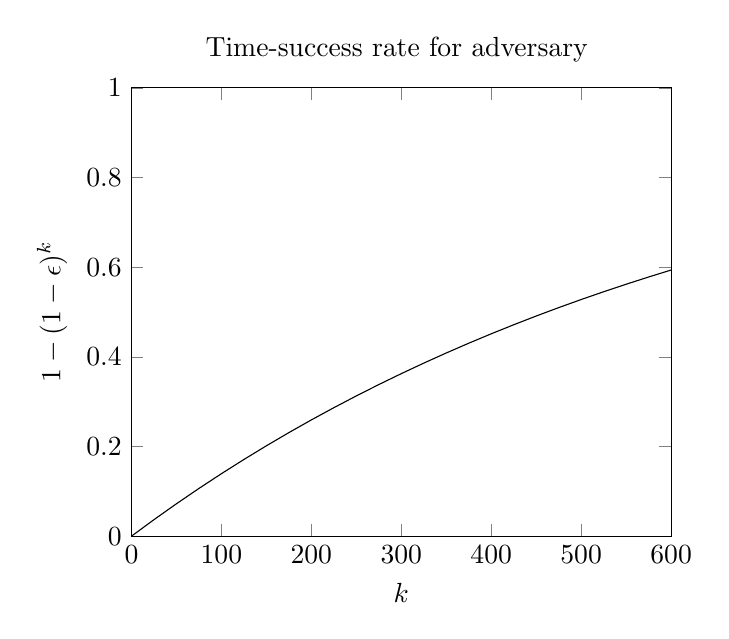
\begin{tikzpicture}
  \begin{axis}[ 
    xlabel=$k$,
    ylabel={$1-(1-\epsilon)^{k}$},
    xmin=0, xmax=600,
    ymin=0, ymax=1,
    title=Time-success rate for adversary $\AD$
  ]
    \addplot[domain=0:600]{1-(1-0.0015)^x}; 
  \end{axis}
\end{tikzpicture}
\end{center}

\end{solution}
\end{document}
